\chapter{Layout
\index{Chapter!Layout}
\index{Layout}
\label{Layout}}
\section{Intro to PCBs}
Before getting into the meat and potatoes of how to design a PCB, I think it is worthwhile to go over the terms and basics surrounding PCBs.
When starting this project I knew absolutely nothing, and probably still do, however it helps to know the terms and have context when
watching tutorials and reading documentation, etc.

\subsection{PCB Layers}

\begin{figure}[H]
  \centering
  \scalebox{.7}{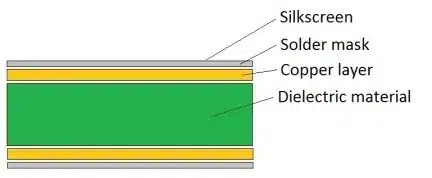
\includegraphics{AllegroImages/layersOverview.jpg}}
\caption{PCB Layers}
\label{img:pcblayers}
\end{figure}

A Printed Circuit Board (PCB) is made up of different materials all stacked up on top each of other, where each of these materials is called
a layer of the PCB. You will also hear the term "stackup" used to describe the amount and kind of layers in one PCB. There are essentially
only four types of layers you need to know, as shown in Figure \ref{img:pcblayers}. The first and most important one is the copper layer.
Copper is a conductor, and so this is the layer in which we place copper where we want to conduct electricity. Whether its for sending power or
signals from one place to another, or placing copper where we want to solder our component pads, this is the place where the actual circuitry is outlined.
You can notice however there are two copper layers in Figure \ref{img:pcblayers}, both of which can have different signals passing through them.
In order to separate the two conductors to prevent shorts, we use a substrate layer, also referred to as a dielectric material. The dielectric
layer goes between copper layers, with one purpose being electrical insulation to keep copper layers from shorting or inducing current in
one another. While it does not conduct electricity, it has a controlled impedance meaning signals won't have weird reactions in different
parts of the board and behavior of signals can be predicted. Different dielectric materials have different dielectric constants, essentially
the number you can use to determine the constant impedance across the board. Now that we have a dielectric and copper layer, we can place a bunch
of copper layers separated by dielectric layers to fit a lot of circuitry in a small space. The third layer we need is the soldermask. The top
and bottom copper layers are exposed to the elements, while all copper layers in the middle are safe within the board. These top and bottom layers
have exposed copper that are subject to things like oxidation, solder shorts between copper areas, and reduces affect of things like moisture.
So, the soldermask is simply a film that goes on top of the top and bottom copper layers to protect it. Finally, the silkscreen layer is just
engraved writing on the soldermask to help humans when assembling the components onto the board. 

\section{Traces and Vias}
\begin{figure}[H]
  \centering
  \scalebox{.7}{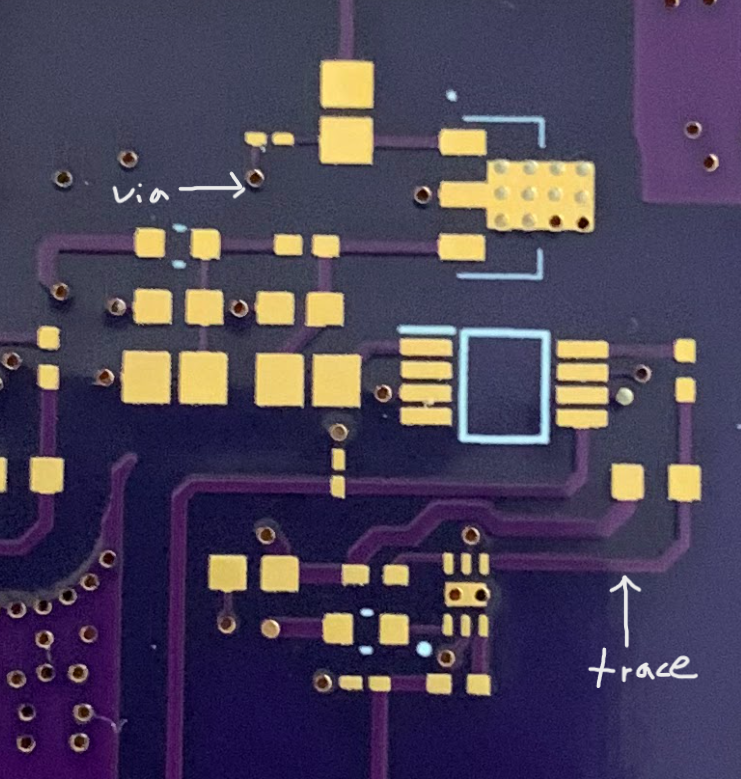
\includegraphics{AllegroImages/tracesandvias.png}}
\caption{Traces and Vias from Mithril Board}
\label{img:tracesandvias}
\end{figure}

In the last section, we mentioned copper layers being where copper is layed down where we want to transmit electricity from one place
to another. This means we have to connect different components, power sources, grounds, etc. with strips of copper which we call traces. As 
can be seen in Figure \ref{img:tracesandvias}, traces can vary in width, orientation, etc., and are basically drawn out by the designer based
on where they want their electricity to go. Their width, orientation, etc. are important, and their affects can be found in Chapter \ref{Radar Theory}.
We also discussed that there can be multiple layers of copper within a board which is great for saving space, but how can we connect one layer
of copper to another when there is an insulated dielectric between them? The answer is vias, which are copper plated holes drilled in the board
that allow for connection of copper in different layers. As can be seen in Figure \ref{img:tracesandvias}, the vias are very small holes which
can vary in diameter and connect to a trace.

\section{Allegro Overview}
\begin{figure}[H]
  \centering
  \scalebox{.4}{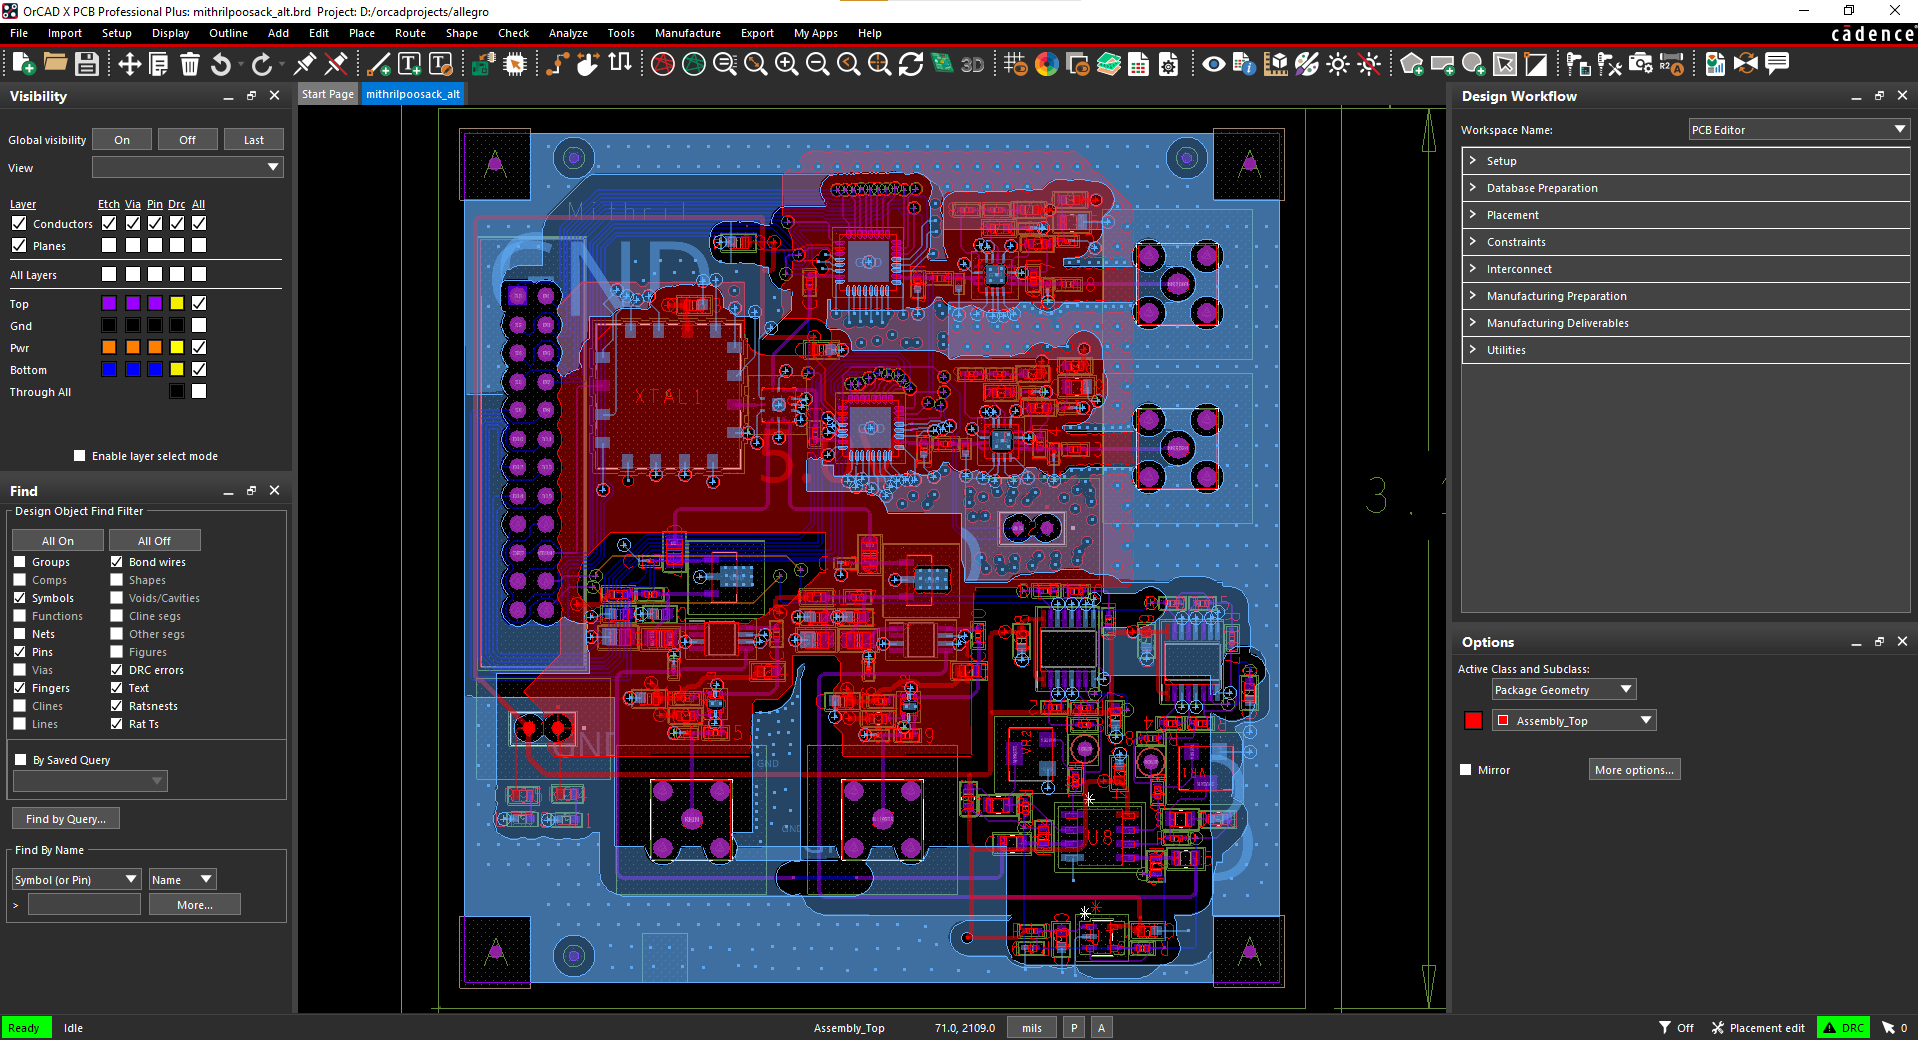
\includegraphics{AllegroImages/layoutfull.png}}
\caption{Allegro Layout}
\label{img:layoutfull}
\end{figure}

First we went over how to create a schematic in Capture CIS, now we will go over Allegro. Allegro is
Cadence's counterpart to Capture which allows you to design a layout for the schematic that can be
printed and assembled to create a functioning printed circuit board.

\begin{figure}[H]
  \centering
  \scalebox{.7}{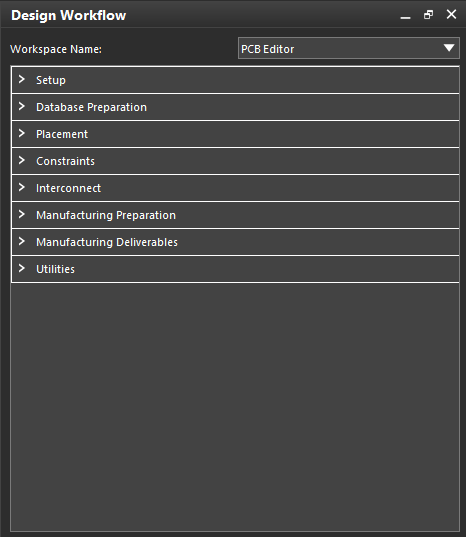
\includegraphics{AllegroImages/designworkflow.png}}
\caption{Design Workflow}
\label{img:designworkflow}
\end{figure}

The most important feature in Allegro is the design workflow. This pane shows all the steps you need to take in order to design a PCB
in Allegro. We will go through all of these panes in the following sections, but make sure to have it open in your Allegro window to quickly
go back and forth from different editing modes.

\begin{figure}[H]
  \centering
  \scalebox{.7}{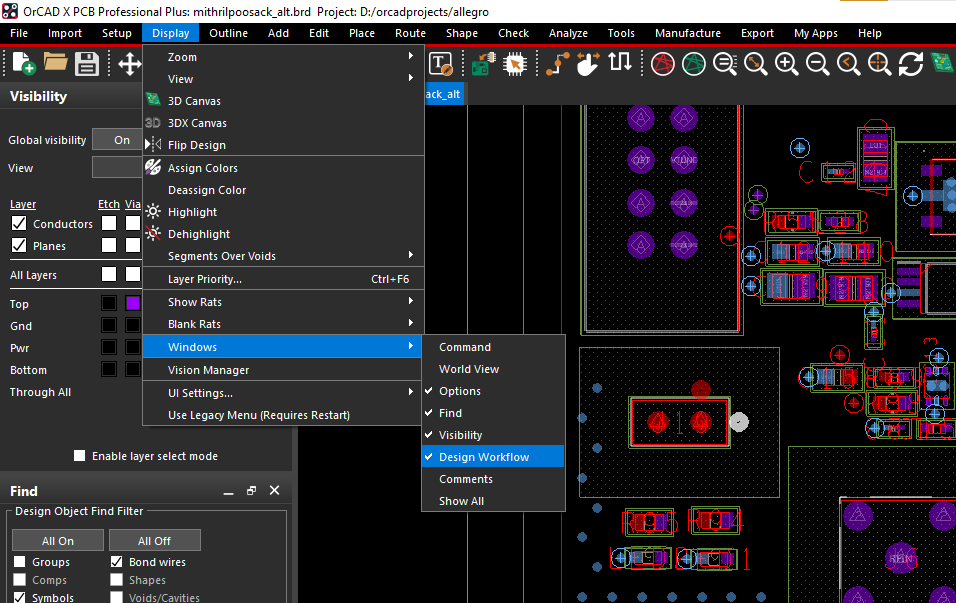
\includegraphics{AllegroImages/windowsTab.png}}
\caption{How to Display Design Workflow}
\label{img:workflowTab}
\end{figure}

If you do not see the design workflow pane in your design, on the top bar navigate to Display, Windows, and then select Design Workflow. You can then drag
and drop the pane to put it wherever you want.

\begin{figure}[H]
  \centering
  \scalebox{.7}{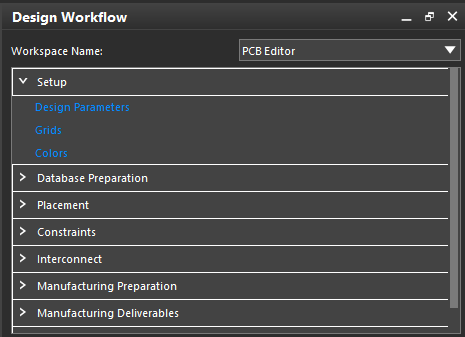
\includegraphics{AllegroImages/setupPane.png}}
\caption{Design Setup}
\label{img:setupPane}
\end{figure}

For Mithril, we followed the design workflow almost verbatim, and this is the workflow we will describe in this tutorial. The first step
is setting up the design to fit our specifications. 

